\documentclass[a4paper,10pt,cours,firamath]{nsi}
\setcounter{chapter}{5}
\usepackage{tabularx}
\begin{document}
\chapter{Opérations bit à bit}
\introduction{cinq et trois font un, cinq ou trois font sept}
\begin{aretenir}
	\begin{itemize}
		\item 	les opérateurs \mintinline{python}{&} et \mintinline{python}{|} procèdent bit à bit et diffèrent de \mintinline{python}{and} et \mintinline{python}{or};
		      
		\item 	on utilise très souvent \mintinline{python}{|} lors d'appels de fonctions qui demandent des flags.
	\end{itemize}
\end{aretenir}
\section{De nouveaux opérateurs}

\begin{center}
	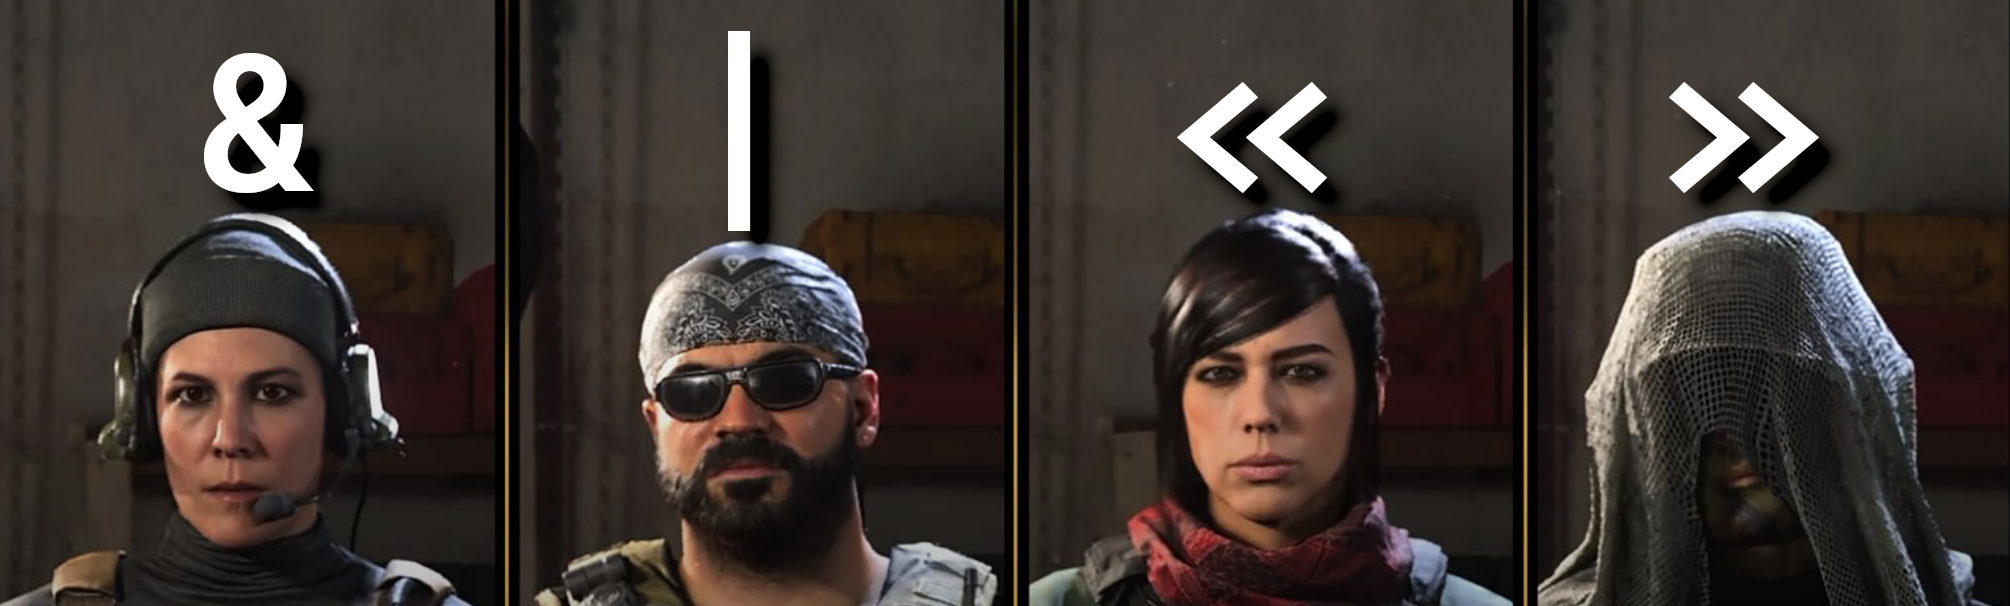
\includegraphics[width=9cm]{img/operateurs.png}
\end{center}
Il n'y a qu'à lire la phrase d'introduction pour constater que « et» et « ou» sont deux nouvelles opérations qui n'ont rien à voir avec l'addition ou la multiplication usuelles.\\
On dit que ce sont des opérations bit à bit (\textit{bitwise operations} en Anglais) car elles se basent sur les écritures binaires des entiers.


\begin{definition}[ : opérateur \&]
	Soient \mintinline{python}{a} et \mintinline{python}{b} deux \mintinline{python}{int} positifs, \mintinline{python}{a & b} est un \mintinline{python}{int} dont la représentation binaire s'obtient en faisant un « et» logique sur les bits correspondants de \mintinline{python}{a} et \mintinline{python}{b}.
\end{definition}



\begin{exemple}[]
	\begin{center}
		\tabstyle[UGLiYellow]
		\begin{tabular}{|c|>{\centering\arraybackslash}m{.5cm}|>{\centering\arraybackslash}m{.5cm}|>{\centering\arraybackslash}m{.5cm}|>{\centering\arraybackslash}m{.5cm}|}
			\hline\rowcolor{UGLiGreen}
			\ccell\'Ecriture décimale & \multicolumn{4}{c|}{\ccell\'Ecriture binaire}             \\
			\hline
			13                        & 1                                             & 1 & 0 & 1 \\
			\hline
			11                        & 1                                             & 0 & 1 & 1 \\
			\hline
			13 \& 11 = 9              & 1                                             & 0 & 0 & 1 \\
			\hline
		\end{tabular}
	\end{center}
	De la même manière, $3=(011)_2$, $5=(101)_2$ de sorte que $3\,\&\,5=1$.
\end{exemple}

\begin{definition}[ : opérateur |]
	Soient \mintinline{python}{a} et \mintinline{python}{b} deux \mintinline{python}{int} positifs, \mintinline{python}{a | b} est un \mintinline{python}{int} dont la représentation binaire s'obtient en faisant un « ou» logique sur les bits correspondants de \mintinline{python}{a} et \mintinline{python}{b}.
\end{definition}


\tabstyled
\begin{exemple}[]
	\begin{center}
		\begin{tabular}{|c|>{\centering\arraybackslash}m{.5cm}|>{\centering\arraybackslash}m{.5cm}|>{\centering\arraybackslash}m{.5cm}|>{\centering\arraybackslash}m{.5cm}|}
			\hline
			\ccell \'Ecriture décimale & \multicolumn{4}{c|}{\ccell \'Ecriture binaire}             \\
			\hline
			13                         & 1                                              & 1 & 0 & 1 \\
			\hline
			11                         & 1                                              & 0 & 1 & 1 \\
			\hline
			13 | 11 = 15               & 1                                              & 1 & 1 & 1 \\
			\hline
		\end{tabular}
	\end{center}
	De la même manière, $3=(011)_2$, $5=(101)_2$ de sorte que $3\,|\,5=7$.
\end{exemple}


\begin{definition}[ : opérateur <<]
	Soient \mintinline{python}{a} et \mintinline{python}{n } deux \mintinline{python}{int} positifs, \mintinline{python}{a << n} est un \mintinline{python}{int} dont la représentation binaire est celle de \mintinline{python}{a}, suivie de \mintinline{python}{n} zéros.\\
	Il s'agit d'un décalage vers la gauche des bits de \mintinline{python}{a}, d'où le symbole \mintinline{python}{<<}.\\
	D'après ce que nous avons vu en première, \mintinline{python}{a << n} vaut \mintinline{python}{a * 2 ** n}.
\end{definition}

\begin{exemple}[s]
	\begin{enumerate}
		\item 	\mintinline{python}{7 << 3} vaut 56.
		\item 	\mintinline{python}{1 << 10} vaut \np{1024}.
	\end{enumerate}
\end{exemple}

\begin{definition}[ : opérateur >>]
	Soient \mintinline{python}{a} et \mintinline{python}{n } deux \mintinline{python}{int} positifs, \mintinline{python}{a >> n} est un \mintinline{python}{int} dont la représentation binaire est celle de \mintinline{python}{a} décalée de \mintinline{python}{n} crans vers la droite avec troncature avant la virgule.
	D'après ce que nous avons vu en première, \mintinline{python}{ a >> n} vaut \mintinline{python}{a // 2 ** n}.
\end{definition}

\begin{exemple}[]
	On veut déterminer la valeur de \mintinline{python}{147 >> 5} :
	\begin{enumerate}
		\item 	on commence par déterminer que $147=(1001\,0011)_2$;
		\item 	on décale de 5 crans vers la droite en oubliant les bits qui passent après la virgule, on obtient $(100)_2$;
		\item 	\mintinline{python}{147 >> 5} vaut donc 4.
	\end{enumerate}
\end{exemple}

\begin{encadrecolore}{Attention}{UGLiRed}
	Les opérateurs \mintinline{python}{&} et \mintinline{python}{|} ne doivent pas être confondus avec \mintinline{python}{and} et \mintinline{python}{or} :
	\begin{enumerate}
		\item 	\mintinline{python}{&} et \mintinline{python}{|} portent sur des \mintinline{python}{int} et renvoient des \mintinline{python}{int};
		\item 	\mintinline{python}{and} et \mintinline{python}{or} portent traditionnellement sur des \mintinline{python}{bool};
	\end{enumerate}
	Ceci dit, \textsc{Python} accepte d'évaluer \mintinline{python}{5 or 3} :
	\begin{enumerate}
		\item 	il évalue logiquement 5, qui ne vaut pas 0, donc est considéré comme \mintinline{python}{True};
		\item 	puisqu'il procède paresseusement, il n'évalue pas 3 et renvoie... 5.
	\end{enumerate}
	
	De la même manière pour \mintinline{python}{0 or 3} :
	\begin{enumerate}
		\item 	il évalue logiquement 0, qui vaut \mintinline{python}{False}
		\item 	ensuite il évalue logiquement 3 qui vaut \mintinline{python}{True} et renvoie donc 3.
	\end{enumerate}
	
	On a le même phénomène avec \mintinline{python}{and}
\end{encadrecolore}

\begin{exercice}[]
	Calculer à la main
	\begin{enumerate}
		\item 	\mintinline{python}{(3 << 5) | (5 << 4) }
		\item 	\mintinline{python}{(120 & 117) >> 2}
	\end{enumerate}
\end{exercice}

\begin{exercice}[ rigoureusement inutile donc indispensable]
	Peux-tu prédire la valeur des expressions suivantes ?
	\begin{enumerate}
		\item 	\mintinline{python}{2 or 7}
		\item 	\mintinline{python}{2 and 7}
		\item 	\mintinline{python}{0 and 7}
		\item 	\mintinline{python}{2 or 0}
	\end{enumerate}
\end{exercice}
\begin{exercice}[]
	On imagine une fonction qui prend (entre autres) en paramètre un \mintinline{python}{int} appelé \mintinline{python}{flags} qui représente 8 flags qu'on peut combiner entre eux comme on le désire :
	pour $n$ compris entre 0 et 7, le flag $f_n$ n'est autre que $2^n$.\\
	Cela veut dire que si par exemple \mintinline{python}{flags} vaut 28, alors puisque $28=(0011\,100)_2$, on a mis $f_2$, $f_3$ et $f_4$ à 1 et les autres flags à 0.
	\begin{enumerate}
		\item 	Comment à l'aide des seuls symboles \mintinline{python}{1}, \mintinline{python}{2}, \mintinline{python}{7} et des opérateurs bit à bit, faire en sorte que \mintinline{python}{flags} présente les deux seuls flags $f_2$ et $f_7$ ?
		\item 	On imagine qu'on a récupéré une valeur de la variable \mintinline{python}{flags}. Comment tester si $f_4$ est bien à 1 ? Comment tester si $f_5$ est à 0 ?
	\end{enumerate}
\end{exercice}

\section{Applications (hors programme)}

Sous Windows, le module \mintinline{python}{pywin} offre un accès à l'API (interface de programmation) \mintinline{python}{Win32}. Celle-ci, destinée à utiliser des fonctionnalités du système d'exploitation Windows, a vu le jour au début des années 90 et a été écrite en \textsc{C} / \textsc{C++}. On peut donc qualifier cette API d'\textit{archaïque}.\\
Dans ce module, on trouve la fonction \mintinline{python}{mouse_event} qui permet de simuler des clics de divers boutons de souris, des déplacements, des glisser-déposer (\textit{drag-n-drop} en Anglais).\\
Voici un morceau de documentation (elle aussi archaïque) de cette fonction :\\



\begin{encadrecolore}{win32api.mouse\_event}{UGLiBlue}
	
	\mintinline{python}{mouse_event(dwFlags, dx, dy, dwData, dwExtraInfo)}\\
	
	Simulate a mouse event\\
	
	
	\begin{center}
		\begin{tabularx}{\textwidth}{|l|l|l|}
			\hline\rowcolor{UGLiBlue}
			\color{white}\textbf{name}         & \color{white}\textbf{type} & \color{white}\textbf{comments}                     \\
			\hline
			\mintinline{python}{dwFlags=0}     & \mintinline{python}{int}   & \textbf{Flags} specifying various function options \\
			\hline
			\mintinline{python}{dx}            & \mintinline{python}{int}   & Horizontal position of mouse                       \\
			\hline
			\mintinline{python}{dy}            & \mintinline{python}{int}   & Vertical position of mouse                         \\
			\hline
			\mintinline{python}{dwData}        & \mintinline{python}{int}   & Flag specific parameter                            \\
			\hline
			\mintinline{python}{dwExtraInfo=0} & \mintinline{python}{int}   & Additional data associated with mouse event        \\
			\hline
		\end{tabularx}
	\end{center}
	\mintinline{python}{dwFlags} controls various aspects of mouse motion and button clicking. This parameter can be certain combinations of the following values.
	\begin{center}
		\scriptsize
		\begin{tabularx}{\textwidth}{|l|l|X|}
			\hline\rowcolor{UGLiBlue}
			\color{white}\textbf{name } & \color{white}\textbf{value} &                                                                                                                                                                                                                                                                                                                                                                                                        \\
			\hline
			MOUSEEVENTF\_ABSOLUTE       & 0x8000                      & The \mintinline{python}{dx} and \mintinline{python}{dy} parameters contain normalized absolute coordinates. If not set, those parameters contain relative data: the change in position since the last reported position. This flag can be set, or not set, regardless of what kind of mouse or mouse-like device, if any, is connected to the system. For further information about relative mouse motion, see the following Remarks section. \\
			\hline
			MOUSEEVENTF\_LEFTDOWN       & 
			0x0002                      & 
			The left button is down.                                                                                                                                                                                                                                                                                                                                                                                                                                                                                  \\\hline
			MOUSEEVENTF\_LEFTUP         & 
			0x0004                      & 
			The left button is up.                                                                                                                                                                                                                                                                                                                                                                                                                                                                                    \\\hline
			MOUSEEVENTF\_MIDDLEDOWN     & 
			0x0020                      & 
			The middle button is down.                                                                                                                                                                                                                                                                                                                                                                                                                                                                                \\\hline
			MOUSEEVENTF\_MIDDLEUP       & 
			0x0040                      & 
			The middle button is up.                                                                                                                                                                                                                                                                                                                                                                                                                                                                                  \\\hline
			MOUSEEVENTF\_MOVE           & 
			0x0001                      & 
			Movement occurred.                                                                                                                                                                                                                                                                                                                                                                                                                                                                                        \\\hline
			MOUSEEVENTF\_RIGHTDOWN      & 
			0x0008                      & 
			The right button is down.                                                                                                                                                                                                                                                                                                                                                                                                                                                                                 \\\hline
			MOUSEEVENTF\_RIGHTUP        & 
			0x0010                      & 
			The right button is up.                                                                                                                                                                                                                                                                                                                                                                                                                                                                                   \\\hline
			MOUSEEVENTF\_WHEEL          & 
			0x0800                      & 
			The wheel has been moved, if the mouse has a wheel. The amount of movement is specified in \mintinline{python}{dwData}                                                                                                                                                                                                                                                                                                                                                                                    \\\hline
			MOUSEEVENTF\_XDOWN          & 
			0x0080                      & 
			An X button was pressed.                                                                                                                                                                                                                                                                                                                                                                                                                                                                                  \\\hline
			MOUSEEVENTF\_XUP            & 
			0x0100                      & 
			An X button was released.                                                                                                                                                                                                                                                                                                                                                                                                                                                                                 \\\hline
			MOUSEEVENTF\_WHEEL          & 
			0x0800                      & 
			The wheel button is rotated.                                                                                                                                                                                                                                                                                                                                                                                                                                                                              \\\hline
			MOUSEEVENTF\_HWHEEL         & 
			0x01000                     & 
			The wheel button is tilted.                                                                                                                                                                                                                                                                                                                                                                                                                                                                               \\\hline
		\end{tabularx}
	\end{center}
\end{encadrecolore}
Les « flags» dont les valeurs sont données en hexadécimal sont en fait des puissances de 2, donc leur écriture binaire comporte un seul bit à 1.\\
Les combinaisons dont parle la documentation s'obtiennent avec l'opérateur bit à bit « ou» : \mintinline{python}{|}.\\
Voici par exemple comment on simule un clic de souris (bouton gauche), puis un déplacement de 100 pixels vers la droite et 15 vers le bas, puis un relâchement du bouton:

\begin{pyc}
	\begin{minted}{python}
from win32api import *
from win32con import *

mouse_event(MOUSEEVENTF_LEFTDOWN | MOUSEEVENTF_MOVE, 100, 15, 0, 0)
mouse_event(MOUSEEVENTF_LEFTUP, 100, 15, 0, 0)
\end{minted}
\end{pyc}

\begin{remarque}[]
	On a utilisé 2 flags lors du premier appel : un pour dire qu'il y a mouvement, l'autre pour dire que le bouton gauche est pressé.\\
	Bien qu'on veuille qu'il y ait ces deux flags en même temps, on utilise un « ou» bit à bit et pas un « et» :
	\begin{tabbing}
		\mintinline{python}{MOUSEEVENTF_LEFTDOWN | MOUSEEVENTF_MOVE} \= vaut \mintinline{python}{2 & 1}\\
		\> vaut \mintinline{python}{0b10 & 0b01}\\
		\> vaut \mintinline{python}{0b11}\\
		\> vaut 3
	\end{tabbing}
	Si on avait utilisé un « et »  on aurait obtenu zéro !
\end{remarque}
\end{document}
